\documentclass{article}
\usepackage[pdftex]{graphicx}

\usepackage[margin=1in]{geometry}
\usepackage{cite}
\usepackage{color}
\usepackage{listings}
\usepackage{pdfpages}
\definecolor{mygreen}{rgb}{0,0.6,0}
\definecolor{mygray}{rgb}{0.9,0.9,0.9}
\definecolor{mymauve}{rgb}{0.58,0,0.52}
\lstset{
  backgroundcolor=\color{mygray},     % choose the background color; you must add \usepackage{color} or \usepackage{xcolor}
  basicstyle=\tiny\ttfamily,          % the size of the fonts that are used for the code
  breakatwhitespace=false,            % sets if automatic breaks should only happen at whitespace
  breaklines=true,                    % sets automatic line breaking
  captionpos=b,                       % sets the caption-position to bottom
  commentstyle=\color{mygreen},       % comment style
  deletekeywords={...},               % if you want to delete keywords from the given language
  escapeinside={\%*}{*)},             % if you want to add LaTeX within your code
  extendedchars=true,                 % lets you use non-ASCII characters; for 8-bits encodings only, does not work with UTF-8
  frame=single,                       % adds a frame around the code
  keepspaces=true,                    % keeps spaces in text, useful for keeping indentation of code (possibly needs columns=flexible)
  keywordstyle=\color{blue},          % keyword style
  language=Verilog,                   % the language of the code
  morekeywords={*,...},               % if you want to add more keywords to the set
  numbers=left,                       % where to put the line-numbers; possible values are (none, left, right)
  numbersep=5pt,                      % how far the line-numbers are from the code
  numberstyle=\tiny\color{mygray},    % the style that is used for the line-numbers
  rulecolor=\color{black},            % if not set, the frame-color may be changed on line-breaks within not-black text (e.g. comments (green here))
  showspaces=false,                   % show spaces everywhere adding particular underscores; it overrides 'showstringspaces'
  showstringspaces=false,             % underline spaces within strings only
  showtabs=false,                     % show tabs within strings adding particular underscores
  stepnumber=2,                       % the step between two line-numbers. If it's 1, each line will be numbered
  stringstyle=\color{mymauve},        % string literal style
  tabsize=1,                          % sets default tabsize to 2 spaces
  %title=\lstname                      % show the filename of files included with \lstinputlisting; also try caption instead of title
}
\title{EEE 178: Homework 3}
\date{\today}
\author{Curtis Muntz}
\begin{document}
\maketitle
\begin{itemize}
	\item Problem 1
	\begin{itemize}
    \item See attached MATLAB code and figures.
		\item Part 6
		\item[] After comparing the differences between the filtered image using the spacial convolution method and the filtered image using the frequency convolution method, it seems as if the spacial filtering was inferior to the frequency filtering. Mathematically, they should produce the exact same effect and the two should not differ. An examination as to why they differ makes me place blame on one thing: mask sizing. In the spacial domain, it is computationally expensive to use a large Gaussian mask, but in the frequency domain, it isn't just easier, it's necessary. Because we use smaller masks in the time domain, it hurts our ability to effectively filter out the noise.
	\end{itemize}
  \item Problem 2
    \begin{itemize}
      \item See attached MATLAB code and figures.
      \item Part 3
      \item[] As we take less and less of the DCT data, since we're still taking data from the `important' region of the DCT, there still exists a distribution. That is | the data still varies in magnitude in an orderly fashion. The top-left most part of the DCT image having the highest magnitude, and conversely the bottom-right most part of the image containing low magnitude values.
      \item Part 4
      \item[] As we take less and less data from the DCT, the image quality suffers, but the `gist' of the image is still there. It is very interesting to see that even using half of the image's data, we can nearly construct the same image, albeit not perfectly.
      \item Part 6
      \item[] The bottom right of the DCT image was taken and scaled lower and lower, and an interesting phenomena was noted. First of all, the data seems to have less variance. that is, while outliers do exist, most of the data corresponds to high magnitude values. Secondly, the data is arranged more randomly. while the magnitude of the data is relatively the same everywhere in this region, the differences are much more sporadic and random, less organized than the data in the `good DCT region'.
      \item Part 7
      \item[] The inverse of these DCT regions produce very unusable images. You can still make out some parts of the original image, in my case you can still see some of the rocket exhaust, but for the most part the image doesn't contain enough information to be recognizable by a human as the original image. 
      \item Part 8
      \item[] Because mathematically the DCT is invertible, inverting the whole DCT of the original image should reproduce the original image. However, because we are taking only portions of the mapping, we are losing some data, and therefore some of the image. When taking the lower right most portion of the DCT, we lose most of the image, but also in the opposite case, we still lose some of the image. This can be seen as the general image degregation between the original image and the iDCT image. While the discarded information obviously wasn't as `important' to the image, it still makes a difference between a perfectly reconstructed image and the lossy `approximation'.
    \end{itemize}
\end{itemize}

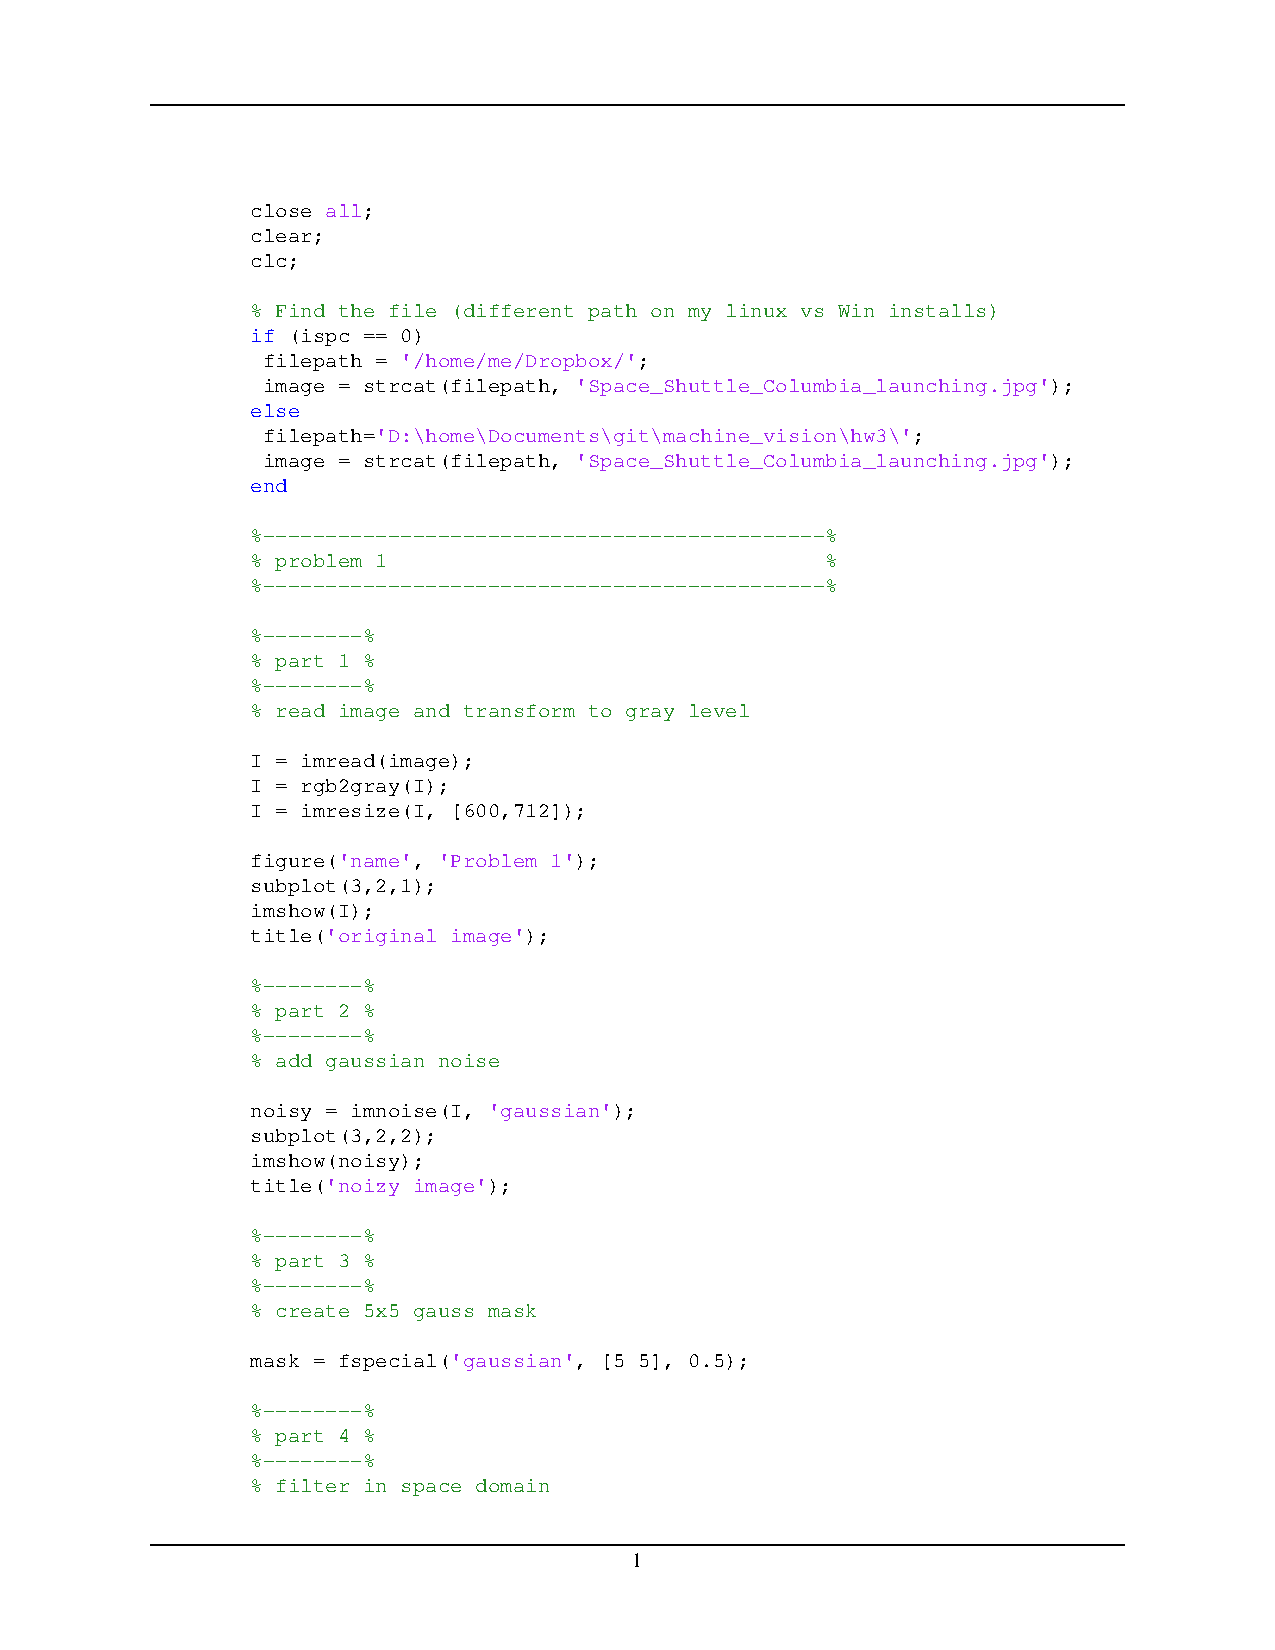
\includepdf[pages={1-8}]{../html/hw3.pdf}
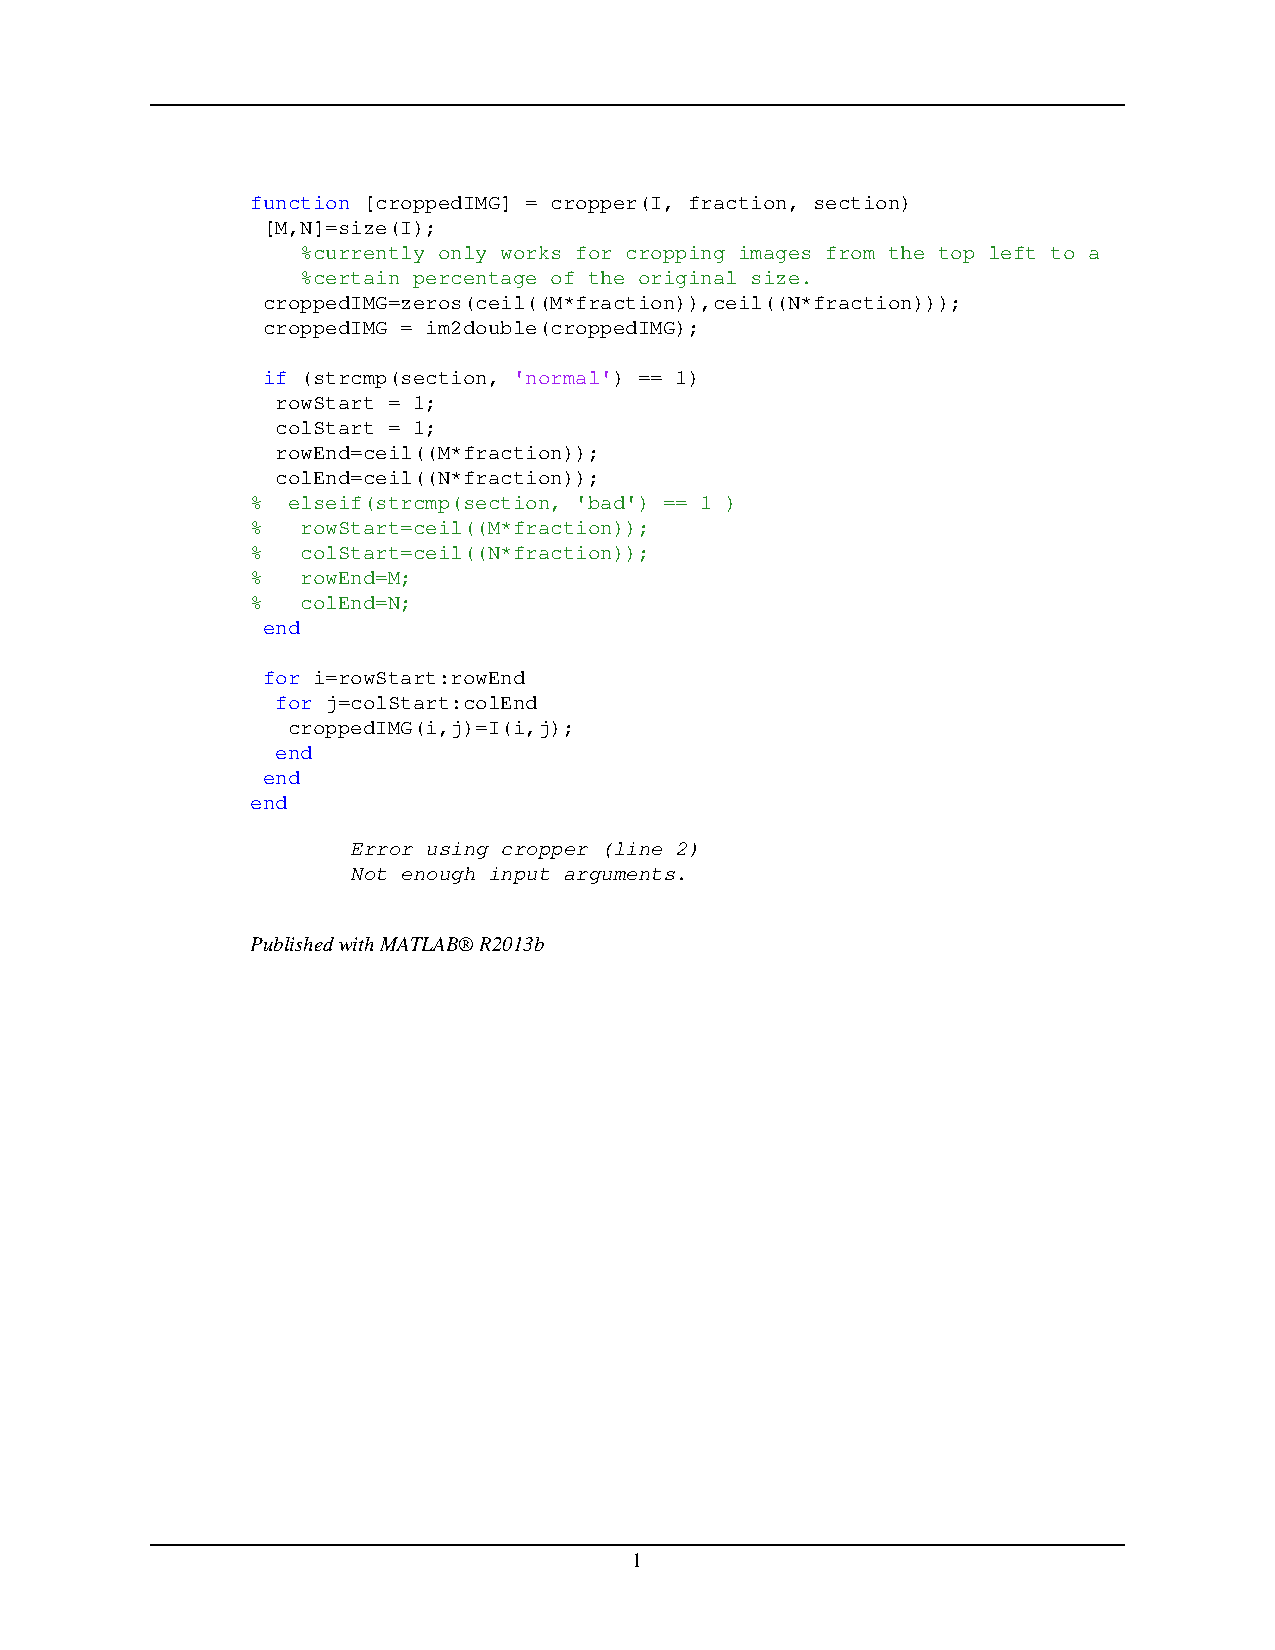
\includepdf[pages={1}]{../html/cropper.pdf}
\end{document}